
\documentclass[letterpaper, 10 pt, conference]{ieeeconf}  
\IEEEoverridecommandlockouts                             
\usepackage{graphicx} 
\usepackage{hyperref}

\overrideIEEEmargins

\title{\Huge Motion Detection Using Simple Image Filtering}

\author{Jiyu Tian} 

\begin{document}

\maketitle
\thispagestyle{empty}
\pagestyle{empty}

%-------------------------------------------------------------------------

\section{INTRODUCTION}
In this project we implemented a simple technique for motion detection and explored various factors that affect the efficiency. The stationary camera capture image sequences where most of the pixels belong to a stationary background and relatively small moving objects pass in front of the camera. In this case, the intensity values observed at a pixel over time is a constant or slowly varying signal, except when a moving object begins to pass through that pixel, in which case the intensity of the background is replaced by the intensity of the foreground object. Thus, we can detect a moving object by looking at large gradients in the temporal evolution of the pixel values.

%-------------------------------------------------------------------------
\section{ALGORITHMS DESCRIPTION}
Our motion detection algorithm is designed to contain 5 steps in total, including 
\begin{itemize}
    \item Grayscale Conversion
    \item Spatial Smoothing
    \item Temporal Derivation
    \item Threshold Selection
    \item Result Generation
\end{itemize}
\subsection{Grayscale Conversion}
After reading in a sequence of image frames, we first make them grayscale. As shown in Figure \ref{gray}, we apply the grayscale conversion as the following eqaution:

\begin{equation}
Gray = 0.299 \times R + 0.587 \times G + 0.114 \times B
\end{equation}

\begin{figure}[thpb]
\centering
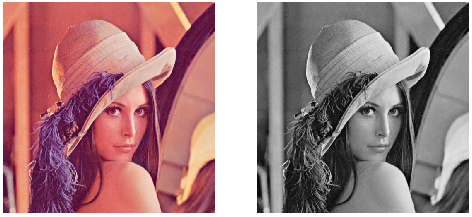
\includegraphics[width=0.46\textwidth]{lenagray2.png}
\caption{Grayscale Conversion}
\label{gray}
\end{figure}
If, in the worst case, some input frames do not have all the $R,\ G,\ B$ values, we simply regard the first channel as its grayscale value.

\subsection{Spatial Smoothing}
The possible bacground noise of original frames could have significant negative effects on accurate motion detection. And thus a 2D spatial smoothing filter is considered to be applied to the frames before applying the temporal derivative filter. Here we tried $3\times3$, $5\times5$ box filters, and $2D$ Gaussian filter with different standard deviation $\sigma$.

\subsection{Temporal Derivation} 
Since the temporal derivatives of each pixel are to be analyzed for large gradients, different temporal derivative filter has different corresponding result. Here we make a comparison between $1st$ and $2nd$ discrete differential as well as $1D$ Gaussian filter with different standard deviation $\sigma$.

\subsection{Threshold Selection}


\subsection{Result Generation}



%-------------------------------------------------------------------------
\section{EXPERIMENTAL RESULTS}


%-------------------------------------------------------------------------
\section{CONCLUSION}


\end{document}

\begin{figure*}[thpb]
\centering
\includegraphics[width=\textwidth]{100sq.png}
\caption{Schematic of topology structure used in the project}
\label{fig100}
\end{figure*}
